\documentclass[12pt]{book}
\usepackage{graphicx}
\usepackage{verbatim}

\usepackage{biblatex}

%% \addbibresource{wacuri.bib}

\bibliography{wacuri}

\begin{document}

\title{Waking Up Curious: The Wacuri Method for deeper connection to self, others, and the Universe (v0.9)}

\author{Brooks Cole, Henry Poole, Robert L. Read, and Dan Spinner}
\date{ }

\maketitle
\tableofcontents


\chapter{Forming Deep Connections}

\section{The Wacuri Method}

The Wacuri Method invokes  you  to a centered higher flow state that wakes you up to curiosity and awe and the Oneness of the Universe. Two or more people go on a 5-minute journey together and then discuss it. More specifically,  a recorded audio or a live person leads you on  journey that strives to awaken the journeyer to awe and curiosity that can be taken into everyday life. In so doing, it forges deep, intimate connections between those participating. A key to the method is the debrief, a discussion afterward of the guided visualization in which each participant has a chance to discussion the impact on their bodily sensations, thoughts, and emotions.


\section{Not Exactly Mindfulness}

The Wacuri Method shares much in common with mindfulness and meditation. Meditation is often lonely; Wacuri journeys are not. Wacuri journeys seek to connect you to the community of consciousness. However, like mindfulness, journeys seek to emancipate you from the tyranny of everyday habit and mind chatter.. Many of us spend each day in a long daydream, dominated by our pasts, futures, to-do lists and our responsibilities. Wacuri seeks to wake us up to the awesome possibilities in every moment. A journey trains you to be present in every moment of your life. It does this by giving you new habits of focus and a witness outside yourself. The transformation of the journey is made more real to you because it is affirmed by your co-journeyers. The meditation is more intense because it is being shared with others. Rather than rejecting society, Wacuri embraces it and asks you to collaborate  and connect deeply with each other. Love is	 the connection many of us feel.


\section{Of Cats and Trees}

A Wacuri Journey is always a journey to something which is not yourself. It may be something inside yourself, such as your inner child, or your relationship with your father. Or it may be a journey to something awesome like a galaxy, or a bumblebee. It seeks awe in both the awe-inspiring and the humble. A journey seeks to give you an intimate connection to something, like a tree or your cat, and to find awe and beauty in that object. Because the journey is co-created, it always gets you outside yourself. You and a friend go somewhere, and your experience strengthens theirs, just as theirs strengthens yours.
				



\chapter{Wacuri Journeys}

The Wacuri Method is a structured approach to a journey. Perhaps
surprisingly, this structure gives great freedom to the journey.
Every journey evolves as a series of acts.
These are:
\begin{itemize}
\item Breathing and Posture,
\item Invitation and Invocation,
\item Introduction to Subject,
\item The Journey Proper,
\item The Moment of Awe,
\item The Space of Appreciation, and finally
  \item The Sharing and Return.
\end{itemize}

All of these acts are accomplished in five minutes, give or take a few minutes. The Wacuri Method compresses an ocean of awe into a limited period of time. Each journey includes a debrief, discussed in the next chapter, an essential part of the Wacuri Method.


\begin{figure}
  \centering
     \includegraphics[width=0.95\textwidth]{WacuriFigures/Wacuri-Journey-Structure-Sky2.png}
     \caption{Journey Structure}
  \label{fig:journey}     
\end{figure}


\section{The Journey Jockey}

In the Wacuri Method, one of the journeyers is the Journey Jockey, a formal role that leads the journey through each act. The Jockey may be a formal
					
teacher or counselor, or may simply be chosen from the journeyers. Like anything, Jockey’s may differ in their skill, experience, and style, but everyone has to start somewhere. If you are reading this book, you are part of the democracy of enlightenment, and with a little training will become  ready to jockey your first journey.
					
The Journey Jockey is the only journeyer who speaks during the first five minutes. In the Debrief, each journeyer gets a chance to share their sensations, emotions, and epiphanies.
					
The Journey Jockey speaks spontaneously from the heart. Although many journeys are educational, the Journey is not a lecture. It is not a purely intellectual expression. The Jockey should use rich, evocative language to try to speak to the body, mind, heart, and even soul of the journeyers. Each journey will play upon different aspects of the human instrument. Some will be more intellectual, some will be more sentimental, some more sensual. The one rule is that a Journey may not be scripted.
					
Some Jockeys prefer to think of themselves as transmitting a journey, rather than creating one. They attempt to open themselves up to the Goddess, or the inner light, or the quiet still voice, or the spirit of peace, and so on. No matter how they do it, they are co-creating the journey with the participants, because the Jockey always imagines themselves to be in the presence of the other journeyers, traveling with them as a guide. The journey is literally co-created with the listeners, even if they remain silent.
					
Let us now consider each Act of the Journey in turn.
					
\section{Breathing and Posture}
					
Every journey begins with a reminder to check one’s breathing and posture. A typical opening is:
					
Be in a quiet spot and take a few moments to adjust your posture and still your breathing. Sit comfortably upright in your chair, or in any posture you can hold for 5 minutes.
					
As in almost every meditative practice, breathing is important, but the Wacuri method prescribes no specific breathing. It seeks merely to make the journey begin with an awareness of their own body–a point of departure if you will–and prepares them to listen intently without interruption for five minutes.
					
\section{Invitation and Invocation}
					
The Jockey then invites the journeyers to join him or her on a journey. The invitation is important because it is just that. The Jockey makes no demands on the journeyers; they are free to decline going on the journey. If they wish they can listen with a certain emotional detachment, without allowing themselves to be transported by the journey.
					
A typical invitation might be:
Come with me on a journey to the Transformation of Fear.
					
Wacuri journeys are supposed to be deep, but any given journeyer may not be ready to go on a journey to the Transformation of Fear of Forgiving Abusive Parents.
					
The Jockey may also make an invocation, a “calling in”, of a spirit, formally or informally. An invocation is often included in the invitation, such as:
					
Come with me on a journey to the Spirit of Nelson Mandela.
					
This formula seeks, figuratively, the guidance of the spirit of Nelson Mandela in the journey.

\section{Introduction to Subject}
					
The subject will probably already have been named, but the Jockey now spends 15 to 30 seconds introducing the subject. Intellectually, this may be a few facts about the subject. Psychologically, it is motion away from the physical surroundings of the journeyer into space of the journey. For a brief time the journeyer is leaving the cares of the day and the world behind. The introduction is meant to begin this process. For many journeyers, it is a welcome release of their own thoughts in order to give their full attention to the Jockey for a brief time.
					
\section{The Journey Proper}
					
The Journey proper is a timeless five minutes. That is, the journey should transport the journeyer out of their normal sense of time. Time is an illusion which is not needed.
					
However, Journeys have space. Sometimes, in the case of a Journey to the Inner Child, this is a change in position from one of maturity and adult responsibility through the long march back to care-free childhood and childlike wonder. In another case, such as Journey to an Owl, it is a physical journey through the chilly moonlit sky vivisected by pine branches and decorated by the noiseless stroke of the owl’s wings seeking the sound or sight of a tasty cockroach or mouse in the mouldering duff of the forest floor.
					
The Jockey should act in the spirit of transmission, rather than in authorship of a story. In fact a Journey is not a story, because nothing need happen. The Jockey should be listening to their heart or soul as it recites the story to the listeners.
					
Nevertheless, the Jockey is not in a trance. Part of their mind is thinking about how the journeyers will perceive the journey. They might, therefore, attempt to enrich the experience by mentioning as many of the senses as possible. A Journey to the Beauty of Fractals might have a little trouble invoking the sense of smell, but in general the more sensual the journey the better.
					
However, the Jockey does not need to cram too much into a journey. Silence gives the journeyer a chance to co-create the journey in their own minds. The oak tree they imagine might not be quite the same as the oak tree the Jockey imagines, but it will be more vivid for the journeyer if they create as much of it themselves as possible. A good rule of thumb might be a 5 seconds pause every 30 seconds.
					
\section{The Moment of Awe}
					
Although it may have several, every journey should have at least one Moment of Awe. This is a moment when the divine is touched, a moment of Apotheosis, or becoming or joining with the Divine.
					
Although there are many benefits to mindfulness and collaboration, the Wacuri Method seeks above all to awaken a sense of awe which can be taken back into the mundane life of the journeyer to enrich it with a sense of the awesome. A stone is a just a stone, but after a Wacuri journey it may be a stone that generates a unique numinous glamor.
					
Although there need not be a single climax to a Journey, the sense of awe should be transmitted by the Jockey. Hopefully the subject is something the Jockey can truly find awe-inspiring in some way.
					
The Moment of Awe is emotionally and psychologically the highest pitch of the journey. It is perhaps the most removed from the need to do the dishes which the journeyer will soon face in one way or another. The purpose is not to emphasize the difference between the Death of a Star and doing the dishes, but to allow the journey to take some of the awesome power of a dying star back with them to the tedious task of doing the dishes.
					
\section{The Space of Appreciation}
					
The penultimate act of the journey of a pause that allows for Appreciation. Possibly there have been several such pauses, but the most powerful journeys may build to a climax of awe and appreciation. This requires space, in the sense that the Jockey must pause and allow the journeyers to appreciate the awesome nature of the subject without the intrusion of their voice. The journeyers should be able to co-create the journey by imagining, or feeling, or thinking, whatever comes from their own hearts at this point.
				
					
Every Journey ends with a brief affirmation of the shared experience and a call to gently bring the consciousness of the listener back into the room and their own body. The return is a coming back to Earth and in some sense the less awesome duties of the day. Hopefully, however, the journeyer will be in an elevated mood, or state or mind, or spiritual level.
					
Many journeyers find this a process that takes 30 seconds or more. It is often the case that the journeyers do not wish to speak for a few moments. In a sense, the gulf between the moment of awe and the return to Earth is so great that it cannot be passed instantaneously.
					
This moment is a sharing because it is a return from the co-created journey to the fact that we are two or three people in a coffee shop or videoconferenced together. We may just have been three seagulls, but now we are people with our own personalities and problems.
				
			
		




\chapter{The Debrief}

The Debrief is a critical part of the Wacuri Method because it allows the journeyers to better integrate the experience and impact of the Journey back into their life.
					
After a suitable coda, the Jockey asks the journeyers to comment on their journeys. This should begin gently and not be rushed. Some journeyers, if there are more than one, will not want to go first.

\begin{figure}
  \centering
     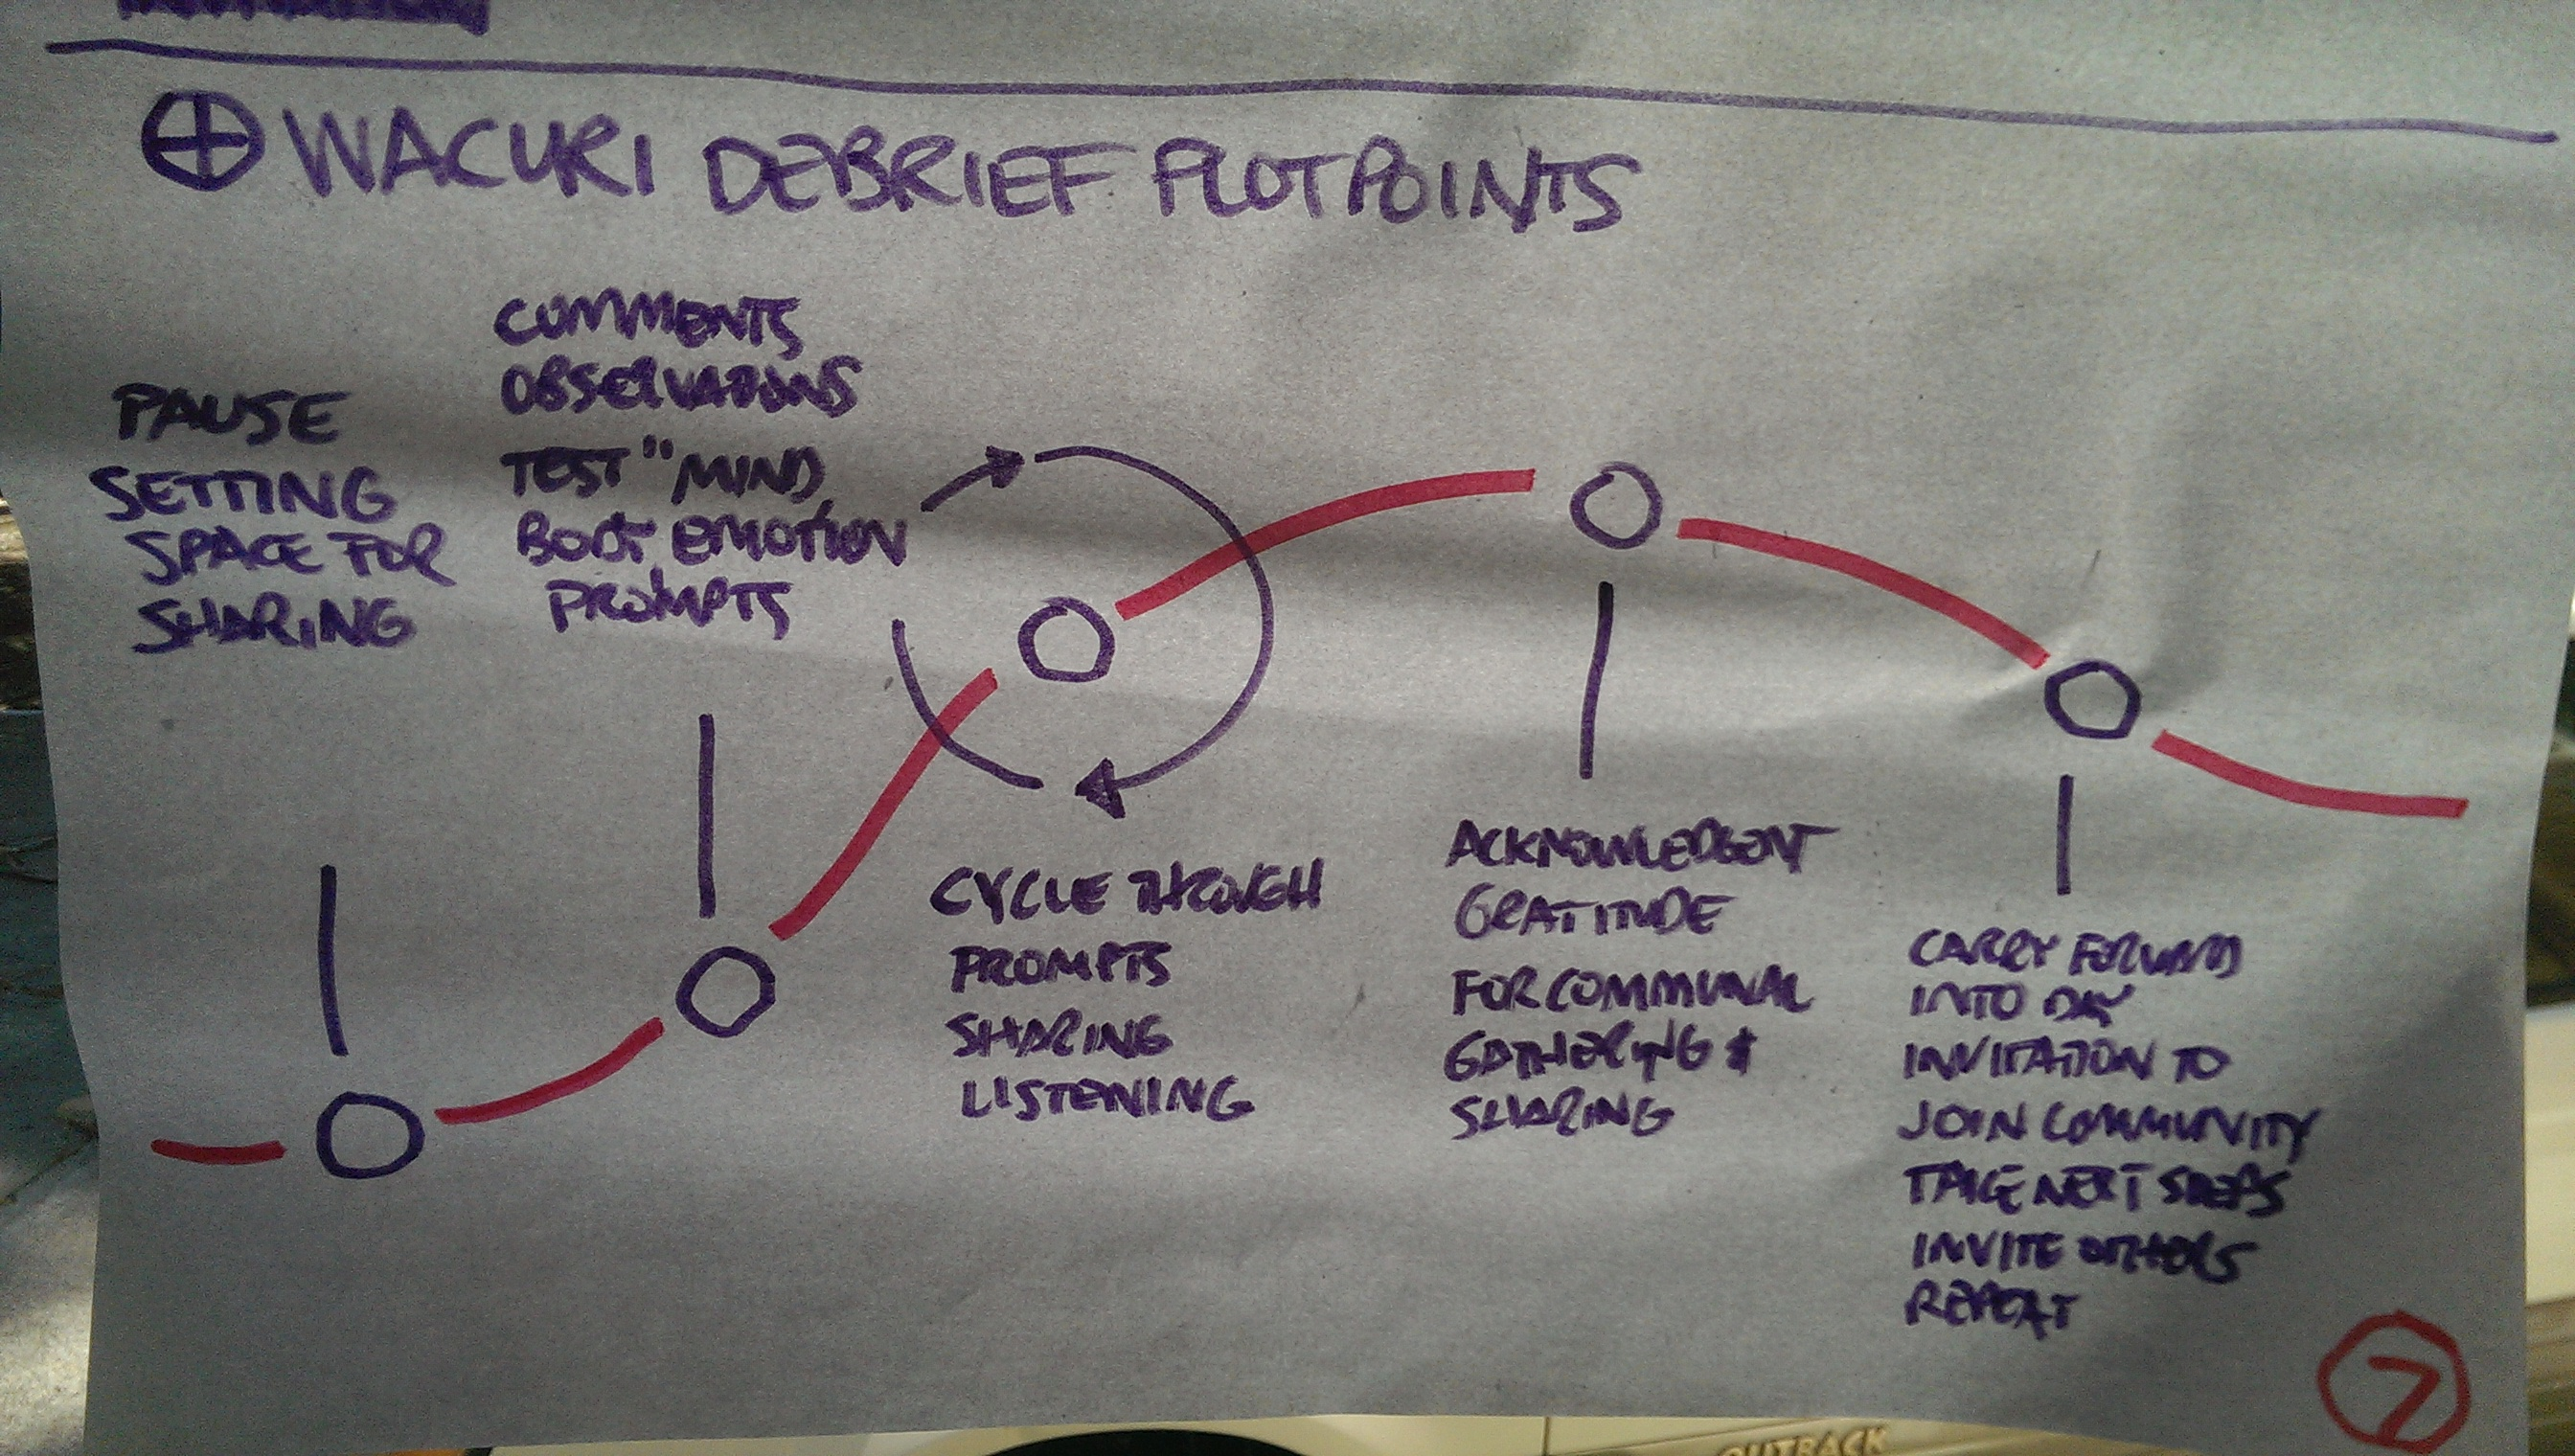
\includegraphics[width=0.95\textwidth]{WacuriFigures/DebriefStructure.jpg}
     \caption{Debrief Structure}
  \label{fig:debrief}     
\end{figure}

Eventually, someone will want to speak about the journey. The speaker is important because it is a psychological affirmation that something has just been shared, both for the the journeyer and the jockey.
					
But as the journeyers describes their experience, they are getting something else of immense value in our world: they are being noticed. Their thoughts matter. The group affirms that they hear and understand their feelings without judging them.
					
Of the authors of this book, some of us are very cerebral, some kinesthetic, and some emotional. All three ways of experiencing a journey are valuable. It is to be expected that not every person enjoys or experiences each journey equally, or at all. It is furthermore the case that some people may be more easily transported than others. It is not a contest in the imaginal realm.
					
The Jockey, if they are comfortable with the other journeyers, may try to elicit an emotional response from the cerebral journeyer, or a bodily sensation from the emotional journeyer, and so on.
					
The debrief is normally between three and fifteen minutes. It is possible that one person’s statement will be a mere fifteen seconds. On occasion, however, the journey will be an intense experience that excites and touches the journeyer, and they will want to discuss it in order to help fix it in their mind.



\begin{figure}
  \centering
     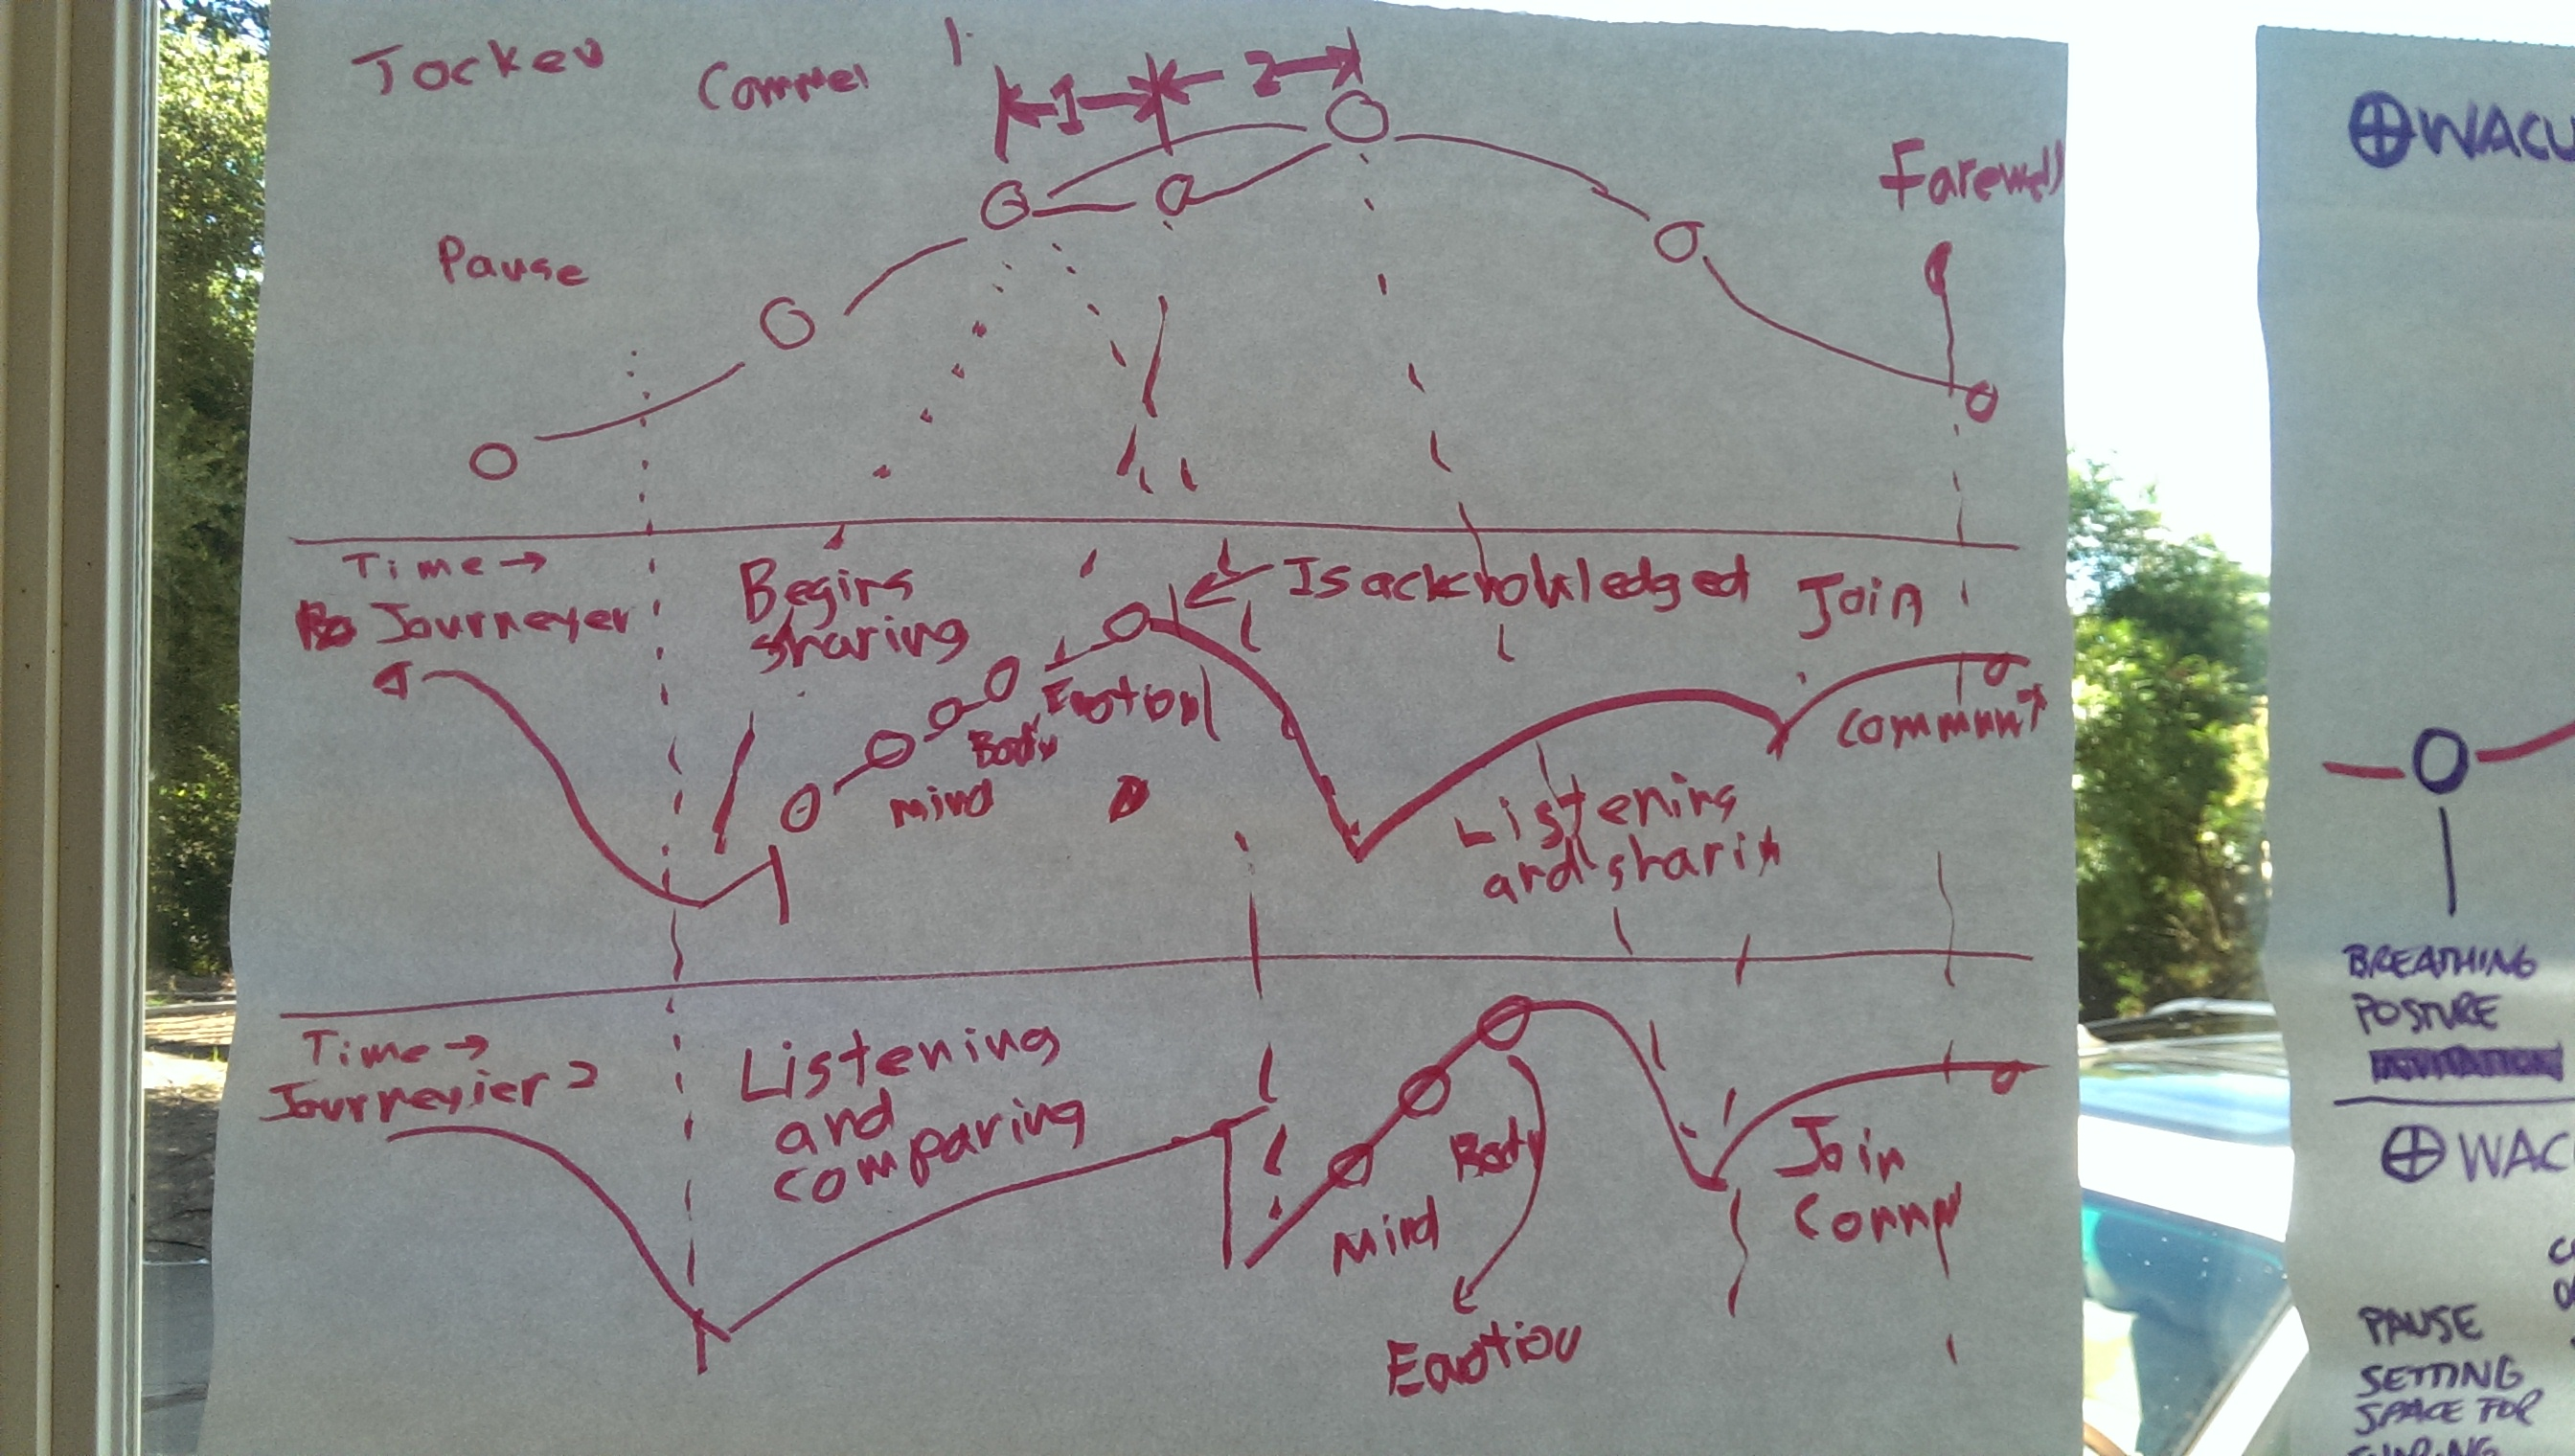
\includegraphics[width=0.95\textwidth]{WacuriFigures/JourneyerInteraction.jpg}
     \caption{Journey Structure}
  \label{fig:journeystructure}     
\end{figure}

The act of discussing the journey, just like the act of keeping a dream journal, makes the journeys more memorable by allowing the verbal part of the brain to register and record the often intense feelings and elations of the journey.
					
In listening to people’s reactions to journeys, each participant gets an intimate glance into the personality, thoughts and feelings of the other journeyers. Even though there is no need for a journeyer to comment on another’s journey, a shared sense of camaraderie is forged. It is often surprising to observe how different another’s reaction can be. When reactions are similar, it creates a sense of like-mindedness.
					
After participating in several journey’s with the same person, you start to feel that you know and understand the other person, and likewise that they have been shown a part of you which you would not ordinarily share with strangers. The fundamental human need to be understood and known is satisfied by this connection.
					
The debrief also gives feedback to the Journey jockey. Although that is not its purpose, it allows  the Jockey to become more skillful at producing impactful and uplifting journeys. This aspect of co-creation further democratizes the entire experience, because the jockey is not seen as an authority figure but rather a performer participating in a closely shared experience.
				
					
The final act of the debrief is a celebration of this shared experience. This recognition that an act has been shared and that each person has spoken and been heard is an affirmation of the impact of the journey which allows the journeyer to carry this short celebration into the rest of their day, hopefully remembering a sense of awe and connected to other human beings.


\chapter{A Sample Journey}


\section{The Consciousness of Cells}

{\em

  Take a couple of deep breaths in your own rhythm.
  
  Adjust your posture to be comfortable.
  
Come with me today on a journey to the Consciousness of Cells. I want		
you to imagine cells throughout your body. A few, a lot. One location, several locations. These extraordinarily tiny, tiny creatures that hold everything that together, that are one of the critical units of our entire structure.
					
Imagine your cellular structure, somewhere in your body, everywhere in your body. Millions upon millions of cells. Interacting, sharing information, nutrients in exchange.
					
And now I want you to imagine that somehow a few of them—just a few—start to light up. In other words, they are aware that you observe them. They lighten up, the light of consciousness. See them perhaps in clusters, in one part of your body or another. Or perhaps many cells, but at least a few. And take a moment now to see your cells lighten up in recognition of you and your growth in your life.
					
PAUSE
					
Perhaps now, the number of cells and the location of cells that are lighting up, that are becoming conscious, or perhaps that you are aware are conscious is increasing. Somehow consciousness begets consciousness. See if your cells now are multiplying their light, feeding one another so to speak, resonating with every light vibration one to another. Feel your body becoming more alive, more alert, as your cells wake up one by one.


And now these clusters of lit up cells are becoming more and more, almost as if there was a rhythm building. in a wave pattern. Feel many more cells lighting up. Somehow connected, communicating with one another.
					
PAUSE
					
And now, they are all lighting up. Every single cell in your physical body— lighting up, celebrating you, celebrating their own awareness. Joining you in your growing awareness, bringing health, clarity, strength and beauty. Just sit soaking that up for a moment.
					
PAUSE
					
Feel the vibrancy of it all. Reaching a peak. Forever changed. Bright, bright as you can imagine.
					
SHORT PAUSE
					
And when you are ready, give thanks, come back into the room, and have a wonderful day.

}

\hrulefill

You have just read a transcript of an actual journey entitled the Consciousness of Cells, jockeyed by Dan Spinner in 2014. The whole journey recording is 5 minutes 17 seconds long. It was performed without a script. Like all such human speech, it is somewhat broken. It is cogent, but does not always use complete sentences. Although it lacks the power of Dan’s voice, we hope the transcript gives you an idea of a journey, although the content varies quite widely. We hope this encourages you to participate or even  try your own.
					
Note also, that although perhaps educational to someone who has not heard of the cellular theory of life, it is not a lecture on biology, but rather a visualization that Dan transmits from his own way of thinking directly to the journeyers.
					
To demonstrate the seven acts of a typical journey, we now repeat the journey, intermixing comments.

\hrulefill
					
					
					
Come with me today on a journey to the consciousness of cells.




\hrulefill

\begin{quote}{\em

    Take a couple of deep breaths in your own rhythm.
    Adjust your posture to be comfortable.
}
\end{quote}

Note here that Dan directs our attention to our breathing and posture to both prepare for the five minute journey and to bring our consciousness into the body.

\begin{quote}{\em
    Come with me today on a journey to the Consciousness of Cells.
}\end{quote}

The Invitation prepare the journeyer mentally and mentions
the subject. The journey may choose to decline the invitation.
In this journey, there is no invocation.

\begin{quote}{\em

I want you to imagine cells throughout your body. A few, a lot. One location, several location. These extraordinarily tiny, tiny creatures that hold everything that together, that are one of the critical units of our entire structure.

}\end{quote}

Here Dan has introduced the subject, which sets the stage and begins transporting the journeyer out of everyday consciousness and into an imagined space. Note that so far the cells are static—they are not doing anything, they are just there.

\begin{quote}{\em
Imagine your cellular structure, somewhere in your body, everywhere in your body. Millions upon millions of cells. Interacting, sharing information, nutrients, exchange.
}\end{quote}
Now the journey is beginning as the cells start to act. The journeyer must use their own imagination to try to picture this.


\begin{quote}{\em
And now I want you to imagine that somehow a few of them—just a few—start to light up. In other words, they are aware that you observe them. They lighten up, the light of consciousness. See them perhaps in clusters, in one part of your body or another. Or perhaps many cells, but at least a few. And take a moment now to see your cells lighten up in recognition of you and your growth in your life.
}\end{quote}

The journey now is fully underway. Hopefully the journeyer is completely transported out of the mundane thoughts of their everyday tasks. This journey is richly visual, allowing the journeyer to exercise their own imagination.

\begin{quote}{\em
  PAUSE
}\end{quote}

To give time to mentally construct this image, the jockey pauses. After a respectful time, Dan begins again:

\begin{quote}{\em
Perhaps now, the number of cells and the location of cells that are lighting up, that are becoming conscious, or perhaps that you are aware are conscious is increasing. Somehow consciousness begets consciousness. See if you cells now are multiplying their light, feeding one another so to speak, resonating with every light vibration one to another. Feel your body becoming more alive, more alert, as your cells wake up one by one.
}\end{quote}


Dan has now brought in a sense of motion and vibration. A somatic
component is added with the suggestion to ``Feel your body becoming...''.

\begin{quote}{\em
And now these clusters of lit up cells are becoming more and more, almost
as if there was a rhythm building.
in a wave pattern. Feel many more cells lighting up. Somehow connected,
communicating with one another.
}\end{quote}

Although Dan mentions no sound, he invites the journeyer to imagine a rhythmic wave pattern, further enhancing the journey. However, Dan never specifies what color the light given off is. To one, it might be white, to another golden, to another different hues depending on where they are in the body. The jockey is not attempting to completely describe the experience, but to transit ideas and feelings. Here Dan once again pauses before continuing.


\begin{quote}{\em
  PAUSE



And now, they are all lighting up. Every single cell in your physical
body---lighting up, celebrating you, celebrating their own awareness.
Joining you in your growing awareness, bringing health, clarity,
strength and beauty. Just sit soaking that up for a moment.
  }\end{quote}

Dan is building to a Moment of Awe. He is brought in an emotion, that of celebration, and the intellectual idea of awareness. Positive imaginations of health and clarity are invited, and then he pauses again.

\begin{quote}{\em
PAUSE

Feel the vibrancy of it all. Reaching a peak. Forever changed.
Bright, bright as you can imagine.
  }\end{quote}


Dan has now reached the Moment of Awe. He is asking the journeyer to imagine as intensely as possible, and slyly suggesting that this change, which is only been imagined, will outlast the the journey as he says “Forever changed.”

\begin{quote}{\em
  SHORT PAUSE
  }\end{quote}

Dan allows the final Space for Appreciation. He gives time for the journeyer to imagine a potentially lasting visual, emotional and intellectual impression.


\begin{quote}{\em
And when you are ready, give thanks, come back into the room,
and have a wonderful day.
}\end{quote}

This is the Sharing and the Return. Dan gives the journeyer permission to take some time, but reminds them to give thanks. He explicitly guides them down from the peak experience back “into the room”, which also means “into your normal, but perhaps elevated consciousness. Finally, the journeyer is asked to “have a wonderful day”, a formula which ends the timeless nature of the journey, in which hopefully normal time has stopped, and restarts the journeyers normal perception of time.


\hrulefill

Note that this journey might not be perfect—in fact Dan himself scored it an 8 on a scale of 1to10. The quality of the journey may or may not be imperfect, but it is better that the journey be genuine and spontaneously transmitted from the heart than scripted. If the journeyers note imperfections in the jockey, it enhances the experience, just as a live music performance is more engrossing than a studio performance, although the studio performance is in a sense more carefully crafted.

\chapter{Sample Debriefs}

\section{Journey to the Consciousness of Cells}

This is a transcript of the actual debrief to the journey “Consciousness of Cells”. Note it demonstrates how quickly the debriefs can be done.


\begin{quote}{\em
Henry: Hmm, I’ll do a quick debrief then I’ve got to jump. I started with some cells inside of my nose, and felt, um, and starting them as bright sparkles, then I felt the spreading and my whole body coming alive in the light and then I felt that extending to people, other people that I know and then extending out to all the trees and animals and the... everything in the universe. I felt all coming to life. It grew from these cells in the end of my nose...
}\end{quote}

Dan: Like Rudolf the Reindeer...

\begin{quote}{\em
Henry: (laughs), yes.
}\end{quote}    

Dan and Brooks: Okay,  see you, Henry, goodbye.


\begin{quote}{\em
Brooks:  The scenes in the Toy Story movies where these
little fluff-ball guys, are kind of a hive mind,
the little alien fluffy creatures are in the machine
with the claw and pray to ``the claw''...
I saw fields and fields of cells on this rolling landscape
that were kind of like these alien creatures because they
were all singing, they were singing in waves and lighting up
you know, the propagation of the light through them went
in waves, in concentric waves, out across the landscape
following the curvatures of the tissues and skins and organs
of which they part. And uh, I just,  I heard the most marvelous harmonic
singing, it was almost like the music of spheres,
coming out of all these little high-pitched voices 
of all these happy cells.
Being so included and transported.
}\end{quote}

Dan: And how do you feel.

\begin{quote}{\em
Brooks: I feel happy, and I feel my uh, my soul is singing.
}\end{quote}    

\section{Journey to the Heart Center}

Dan: “You want me to do it again?”
Adam: ...you know I don’t thank that is necessary, I think I got the
					
transmission. I noticed that my heart center it didn't have a, uh, it had a certain density in the middle, that went further in, it got more dense, there was no real delineation like it moved out past my shoulders out in front of me, beside me. Kind of whitish in color on the outside and yellowish where it became more dense. Certainly interacted at the same beat that physical heart was beating. Certainly gave me a feeling of warmth and a certain feeling of being connected to other people, not all things, but other people.
					
“What would you say your emotional state was or is?”
					
Very calm. When you said think of someone you love I noticed that swirls of red and blue, like sort of Pollock-swirls, went inside of it and like, um, a combination of joy and sadness without thinking of anyone in particular.
					
Dan: “Yeah. Henry?”
					
Henry: When I went there, I thought, it kind of started out as white, and it quickly turned green, kind of green glowing, like kind of sphere, but kind of a star though with points coming out at 90 degrees all the way around, coming out on the top and bottom, kind of like a star. It kept changing colors too to yellow and blue and becoming larger, and um, and it was pulsing similar I think to my heart, as well. It got larger, larger than my body, larger than the planet, I felt like it was out beyond the universe, heh, it just seemed like was everything.
					
When I thought about Maria’s energy and her heart, I got to think about somebody... love her, I just, I felt it, um, I felt calm, I still feel calm. I feel like I’m floating. In joy...it’s kind of a joy feeling of just being connected.

Thinking about bringing it into my day, I’m like, just awe, yeah, I like that, I like that, I want to see that, I want feel that.



``I should have known Henry when I found myself saying make it has large as you want,
you would make it as large as the universe, heh heh.''


Dan: And you know, when we practice these centers, this one and other, another act of integration, taking the energetic aspects of our beings, exploring them and integrating with our psyches and our physical bodies, and so the act of taking into the workplace or with a loved one, either in or near our reality or imagination changes things. For example, just try to imagine if you can, being in your heart center and being mad at someone. Or annoyed. Um, it won’t happen.
					
Well the other way of being annoyed or mad at someone but opening up your heart center for the annoyance or anger. When that other person colleague, friend, partner, learns about the heart center, then good for them, then think about, just as you implied Henry, think about the power doing that with your family of your kids. Imagine teaching your kids about the heart center. There are many, many applications, it’s just fun to explore.


Dan: Other comments or questions for one another?

LONG PAUSE

Adam: Nothing is coming up.

Dan: Think about your own relationship. And the homework is to try it. Just play with it. Maybe when you are in a pretty good place,
but when you are not in a good place, you might want to try it to.

Dan: How are you each feeling now?

Henry: I'm feeling you know, just sedate.

Adam: Pleasant and a little bit excited to try this out both with my daughter and with a couple of friends of ours.

Henry: Maybe I'll try it with one or both of my boys.




\chapter{How to Use Journeys}


Create a way of measuring and talking about deep connections. Wacuri is an algorithm for deepening connections. Want a new glossary and words for the formation of connections. Note: Consider adding here something from Aneels' neurobiology of relationships frame work ( I am looking for any article he may have written on this)

Image of person as black hole becoming a field of stars. Create good stories for this

Create a ability to measure growth through healing or for specific purpose. Analyze language of debrief.


Analyze language of debrief.

\chapter{ A Multiverse of Journeys}

Many traditional mindfulness practices recommend performing the same exercise every day. The Wacuri Method supports the spontaneous creation of new subjects each time, within the basic structure of the method. Journey participants are free to take entirely different Journeys each time or to repeat Journeys they like in any manner they want.
					
Although this lack of discipline or single minded focus may at first seem a weakness, we have found it to be a strength. Unlike a mindfulness practice that seeks “one-pointedness” or to still the thoughts completely, the Wacuri Method encourages rich exercise of the mind using the imaginal spaces. Like traditional mindfulness, the journeyers experience is non-verbal until the debrief. The jockey, of course, is constructing a verbal experience.
					
If this is indeed a strength, we suggest you explore it fully. There are no limits to the subjects of the meditations. We often use objects or animals, such as a Bumblebee or a Spider web from nature because they tend to invoke awe. One of of the authors (Rob) is a computer scientist who sometimes does journeys to abstract, non-physical subjects such as the Realm of Mathematics. Some of our most powerful journeys are psychological, such as Journey to the Inner Child or Journey to the Transformation of Fear.
					
By celebrating the diversity of such subjects, it is necessarily the case that not every journey will resonate with every journeyer. In general each of us takes varying of pleasure and exhilaration along different dimensions of our psyche from each journey. Not every experience will be a peak experience. Sometimes in the debrief we express that the journey was mildly interesting only to discover that the same journey riveted another journeyer, perhaps due to their past experience or a difference in their personality.
					



Appendix \ref{sec:journeys} lists some of the journeys which we have actually produced. However, feel free to use these topics yourself. Your understanding of Dark Matter or the Inner Child may be completely different than ours. Because journeys are not lectures meant to convey scientifically accurate information but rather artistic explorations, it is not particularly important that a journey cover or not cover a particular topic. The value of the journey lies solely in its experience and effect.

\chapter{Origin of Waking Up Curious}

In early May, 2013, Dan Spinner was in Victoria Canada and became curious about using technology to improve and broaden his Life coaching practice by using modern technology. While meditating, he visualized collaborating with experts.
					
At the same time, several hundred miles south in Lafayette CA, Henry Poole was becoming curious about bringing mindfulness practices into government. Henry had just met with executives at the FCC and Census and felt that the modernization of government technology was hindered by corporate and bureaucratic culture. Adopting new technologies was crippled by the intransigent, hardened, blame-oriented institutions within the Federal Government.
					
On May 9th, 2013, Henry called Dan to discuss possibilities to transform the culture of the US Federal Government.
					
Henry told Dan that he was trying to bring enlightenment to, of all places, the US government. Dan shared his interest in increasing the impact of his work through emerging technology. At that moment, Henry and Dan began weekly calls to brainstorm ideas. They discussed the need for a new language, new tools, and new science. They became very excited about the possibilities. Not long afterwards they invited Brooks Cole to join the discussions.
					
Looking for ideas to transform government, Henry and his board at Civic Actions had also recently enrolled in a course at the Google spin-off - Search Inside Yourself Leadership Institute (SIYLI). SIYLI had developed a very effective methodology for increasing the productivity of programmers by teaching meditation practices. One of Henry’s key takeaways from the SIYLI training was the interest in Curiosity.
					
During the weekly calls with Dan and Brooks , Henry became clear that the struggle that federal government employees were experiencing, while much more aggravated, was similar to his own. He felt too busy to keep up his daily meditation practice. For Henry, the logic and obvious benefits weren't enough to get out of his personal daily busy habits. He knew the benefit of a daily practice would pay for itself immediately...but just couldn't break his habit of back to back meetings, endless ToDos and dealing with two boys entering their teenage years. Brooks agreed.
					
He asked Dan to coach him, with a difficult limitation: he wanted to do five minute meditations. Furthermore, Henry needed a coach or a mindfulness buddy, much as people need running or lifting partners, to make them more likely to do their training by adding the peer pressure and social facilitation of doing something collaboratively. Few people will let a partner down by not showing up nonchalantly.
					
Dan was a life coach who had meditated for years in the 20 minute or more style. In fact, there is an unstated belief in the mindfulness community that “more hours makes you a more better person.” Five minutes was quite a departure for his traditional practice.
					
In several of the weekly meetings, Dan, Brooks and Henry discussed this 5 minute requirement. Henry knew that he just wouldn't commit to a longer block of time. Dan wasn't sure that he could do it but agreed to give it a try.
					
Dan rose to this challenge by employing one of his firmly held convictions: that time is an illusion. Perhaps the twenty minute rule-of-thumb was a guideline that could be questioned. By not planning or scripting the meditation but rather spontaneously transmitting the visualization, they found that they could make an effective journey in only five minutes. Dan had always asked the groups he coached to comment on their meditation experience, but now, because Henry needed a meditation partner, they realized they could make the debrief an essential part of every mindfulness training session. Although begun as a crutch for a busy executive, it turned out that having a person there to share the experience deepened the experience by forcing both a human connection and a verbalization of the experience.
					
For years,  Henry, Brooks and Dan had been practicing meditation. They all noticed that a regular practice of meditating brought almost magical connections into their life. They both noticed that maintaining a calm state of centeredness brought more frequent high quality insights. There was a clarity that emerged, where their decisions seemed more accurate. They became more curious.

					
They had also all  experienced lucid dreaming. A lucid dream is defined in wikipedia as ”a dream during which the dreamer is aware of dreaming. During lucid dreaming, the dreamer may be able to exert some degree of control over the dream characters, narrative, and environment. Henry had a desire to bring aspects of lucid dreaming into his waking state. What he wanted now was to wake up from his tedious overfilled day. Just as one can wake into a dream and realize one has the power to fly, or change the grizzly bear into a teddy bear, or to do anything in the dream state you want, so to can a person wake up in their daily life and realize that they are not imprisoned by their todo lists and meeting schedule? Responsibility does not preclude freedom.
					
One of the techniques used by lucid dreamers is to create a personal anchor that once observed in a dream, will trigger the dreamer to see that they are observing the dream. That anchor puts the dreamer is a state where they are aware of their power. Henry thought that perhaps the waking state could be similarly hacked. Maybe the busy life of never ending thoughts could be interrupted by a noticing that he was not his thoughts. Maybe practicing quick meditations could create some similar anchor where he could wake up to curiosity in daily living.
					
Perhaps, one can wake up to vast potentialities in normal life. The name Wacuri is a portmanteau of “Waking Up Curious.”
					
Dan, a student of traditional enlightenment practices, knew this as stepping into the unknown, and used it in several ways in the Wacuri Method. For example, in the semiweekly meeting of the founders of Wacuri, the person who will be the jockey and the topic of the meditation is chosen spontaneously, on the spot. Sometimes the jockey does not choose the topic. By nonjudgmentally allowing a spontaneous journey, it is possible to have an effective, if sometimes fumbling, collaborative meditation. This spontaneity requires the Journey Jockey to be very present in the moment and let the Journey emerge from the deepest parts of their Being.
					
Through subsequent several years of practice, the Wacuri Method was developed into a set of best practices and guidelines presented here. The system fundamentally was born from the necessity of a personal growth system applicable to busy executives.
				
			
	

\chapter{Stories}

\section{Light in the Face of Mortality, Wisdom in the Face of Death}
					


It’s a warm summer day in a hot inauspicious, church meeting room. About 30 women are gathered around sitting quietly in a circle. Very quietly. They all have cancer. Some in very advanced stages, others in remission, still others mid diagnosis in the agonizing in between time. 

They range in age from the very young early twenties to the seventies. They are very quiet but very present. As a Vice President of the local Hospital where most receive their care and treatment and a long time meditation teacher, I have been invited to lead a meditation with this group. I feel totally inadequate and humbled in the face of both their suffering and their courage.

 I tell them that and then we proceed to do a “check in” – that is we go around the circle for those that want to say something to the group about why they are there and how they are doing. It is even more humbling, almost overwhelming for me as the only “healthy “one in the room.

Their circumstances and challenges are presented in a matter of fact and mostly neutral tone. One young lady tells us that she’s going blind, another older one that she is at stage four and doesn’t have long to live. Others describe elements of their battle, still others talk about their families and loved ones.

All speak with a courage and wisdom I cannot fathom as the so called “expert “in the room.  I do my best holding back tears of admiration and compassion and lead the group in a meditation. They take to it amazingly quickly and suddenly the room is full of an ineffable Light I have only occasionally ever felt.

They have all faced death imminently or knocking and threatening at the door. For the most part, they are rising above it to a higher plane of existence and reality. The flow of conversation when we debrief the meditation is easy, relaxed and enlightening. At least for me. Years later, when I face my own battle with an advanced and aggressive cancer, I use the memory and taste of their casual wisdom and Light in the face of disease and death that seared into my being that day to guide me to my own Higher place. I am so grateful for the Better Angels of their Being and it becomes a guiding Light for me for the rest of my life.


\section{Imaginal Calisthenics}

Brook's personal experience strengthening imagination through practice.

\section{Henry's Experience}

Placeholder 

\section{A Field of Stars}

A fictional story about someone moving from lonely to connectedness via journeys.
\chapter{The Wacuri Method and Technology}

Technology seems to be disconnecting and trivializing our human relationships.
Wacuri seeks to reverse this by focusing on human connections. The Wacuri method
insists on the ``debrief'' as a necessary human interaction between two or more people.

However, Wacuri is also seeks to use modern technology to connect people.
The most obvious technological approach is to use recorded audio Journeys.
However, we have have also used videoconferencing to allow us to experience live journeys.

Technology can be used to give as many people as possible the Wacuri experience.
Because the Wacuri Method extols the advantages of partner-based journeying,
one has the same problem finding a meditation partner than you do having a
workout partner. You also get some of the same social benefits of motivation,
if you and your partner can successfully schedule periodic journeys.

Just like a dating app, technology can be used to match meditation partners.

Similarly, technology can help solve the difficult problem of scheduling an
acceptable time between two or more busy people, even when that time is only fifteen minutes.

More importantly, technology can deliver audio recordings of Journey's by
experienced Journey Jockeys. Although we enjoy a live a experience and hope
everyone gets to participate in Journey's presented live, we know that we
can reach more people through recorded journeys.

In a recorded journey, the Jockey is not ``live''. However, it is
important that the participants have a live experience of each other.
Whether that is by traditional phone, computer-based audio, or computer-based
video, it is important that the participants feel a sense of ``togetherness''.
We therefore prefer live video conferencing such as that provided by Skype,
Zoom, and Google Hangouts. Furthermore, as a best practice, participants
should leave their cameras and audio on, even if they are not speaking or
moving during the Journey.

The debrief of course requires shared audio, and benefits from shared video.
You want to listen as deeply to each participant as possible.

Wacuri is currently seeking investment to allow us to create a software
product that solves these problems of finding a buddy, scheduling a time,
and hosting the Journey and the Debrief.

Additionally, a perfect system would allow sophistication selection of
the Journey or even a live Jockey. It would keep a record of the Journey,
including an audio record of the debrief for future reference. We would
also like to explore biometrics, such as pulse and breathing rate, and
well as direct measurement of brain waves.


\chapter{Transmission}


The Wacuri Method requires at least two journeyers. One person creates the spoken Journey and it called the Jockey.
					
To our way of thinking the Journey is not written but transmitted--which might be define as the sharing of feelings and energy with the listener. A Journey is a performance, not a composition. The Jockey attempts to let the topic of the meditation become the source of the feelings, thoughts, and impressions which make up the journey. This chapter is devoted to explaining this process and giving some of the best practices and techniques we have learned to help you Jockey your own Journeys.
					
The goal of being a journey is to awaken curiosity and if possible awe in the journeyer. You could do this by writing, or by drawing, or with a photograph. However, the Wacuri Method uses a different technique. Rather than using the practices of creative writing, or slam poetry, or oral storytelling, all of which are beautiful and powerful arts, the Wacuri Method sees the Journey as flowing from the source of the topic through the Jockey to the journeyer in a process called transmission.
					
In this process, rather than intellectually constructing a spoken-word experience, the goal is to authentically convey with minimum artifice the thoughts, feelings, and awe of the source directly. It is perhaps closer to a jazz improvisation than playing from a written piece of music.
					
To do this, the Jockey should center themselves and attempt to obtain a so-called flow state. It may help to invoke something larger than yourself. You then open yourself to the topic of the meditation. At that point the topic becomes the source—the active subject of the meditation, and the source of the conveyed or transmitted thoughts, adumbrations, impressions, sensations and feelings.
					
If the source is a tree, the jockey should try to feel the tree intensely. A practice that sometimes help is to recall the most intense memory you have of a tree—--perhaps a favorite tree that you climbed as a child. You should try to connect deeply  to the feeling of the tree. If the object is something of which you can have no direct experience, such as a black hole, you should still try to connect to the imagined power, energy, majesty and danger of a black hole. It is better to do this without verbally listing too many aspects of the tree or black hole in your mind. You are not about to compose a lecture, but to transmit impressions from the source.
					
The may be emotionally challenging as well as mentally difficult. For example, if the source is the Transformation of Fear or Recovery from Addiction, the jockey must feel the fear or chains of compulsion, and be prepared to convey that, hopefully before conveying relief from the fear or emancipation from compulsion.
					
After mentally connecting to the source, the jockey must connect to the journeyers. Even if making a recording, the jockey must imagine the journeyers and begin to see themselves as a conduit or vessel for transmission from the source to the journeyer.
					
Trying to feel both the source and journeyer, the jockey is ready to begin.
					
We have already outlined the basic structure of the journey, which should be considered an important guideline. However, other tips to keep in mind include:
					

	\begin{itemize}
\item 

Invite your journeyers to vividly connect to the source. It may help to use language that mentions the senses and emotions or the psychological structure of your journeyers.
						
						 					\item 		
Frequently give the journeyers permission to construct their own version of the source by saying “You choose...” or “You pick...”. Precision quickens writing, but is not needed in transmission, though you may find yourself giving precise details, while leaving some aspects of the source unspoken or unspecified.
						
						 					\item 		
Try to transmit partially verbally and partially emotionally. It is not necessary to reduce all information to words. Beginning Jockeys  generally find the source gives them an avalanche of words that far exceed what can otherwise  be transmitted fully.
						
						 					\item 		
Silences are golden and necessary. Pauses are needed for your journeyers to have time to connect to the source in their own imagination.
Pauses also give you a chance to sense the strongest impression to transmit from the source.

\item 
Fill silences with emotion, not sound. When you pause, you should still feel your connection to the source as compellingly as possible and imagine this same connection to your journeyers.
\end{itemize}
  
					
Just as you should love someone not just when you say “I love you!”, but before and after this exclamation you should try to connect to your source and journeyers ahead of time and follow through with some mental energy after the journey. This does not have to be specific. For example, you may not know the topic ahead of time, but you can still imagine a successful connection between the source and journeyers.
					
Finally, you may want to watch for delightful surprise as a marker for your success. If in a journey to a Flower you find yourself delightfully surprised by something you have said that appears unplanned, perhaps the life of a spider residing in the Flower, this may be a sign that you have achieved the spontaneity of flow that you are seeking.
				
			
\chapter{Curiosity}

Wacuri seeks to awaken people to more presence in their daily lives so they are more curious about and aware of things they may once have taken for granted. Journeys may remind people of and restore them to the child-like wonder about life that they once knew. Wonder and curiosity encourage deeper connections between people and the objects of their curiosity.
					
Ideally you should be curious about the journey, your journey partners, and yourself. Curiosity dissolves the ego. Overtime, journeys strengthen the “curiosity muscle”, which can be found working in opposition to the self-centeredness muscle. Mindfulness subtracts distraction, Wacuri adds curiosity, which is contagious and addictive.
					
In order to be curious, people must feel safe. The jockey and the journeyers must support in each in creating an emotionally safe environment. For this reason, it may be that the best number of participants for a journey taken with strangers is only two or three people. Everyone seeks connections to other people, when they are able to manage the risk associated with forming those connections. The journeyers should all help each other to feel and be safe.


\chapter{A Journey Journal}

Experience cannot be reduced to a number.  Nonetheless, just
as many athletes keep a training log, some people will find
keep a Journey Journal a pleasant and informative experience.
We recommend simplicity. Every entry in the Journey Journal
needs only five items:
\begin{enumerate}
\item the date,
\item the journey title,
\item a selection of words from a mood circumplex that
  describe your mood,
\item a number between 1 and 10 representing the quality of
  the journey experience, and
\item a free-form field where you can write any comments
  you want about the journey.
\end{enumerate}

You may choose to select one or more words from a standard
emotion circumplex like that shown in Figure \ref{fig:emotionwheel}.
\begin{figure}
  \centering
     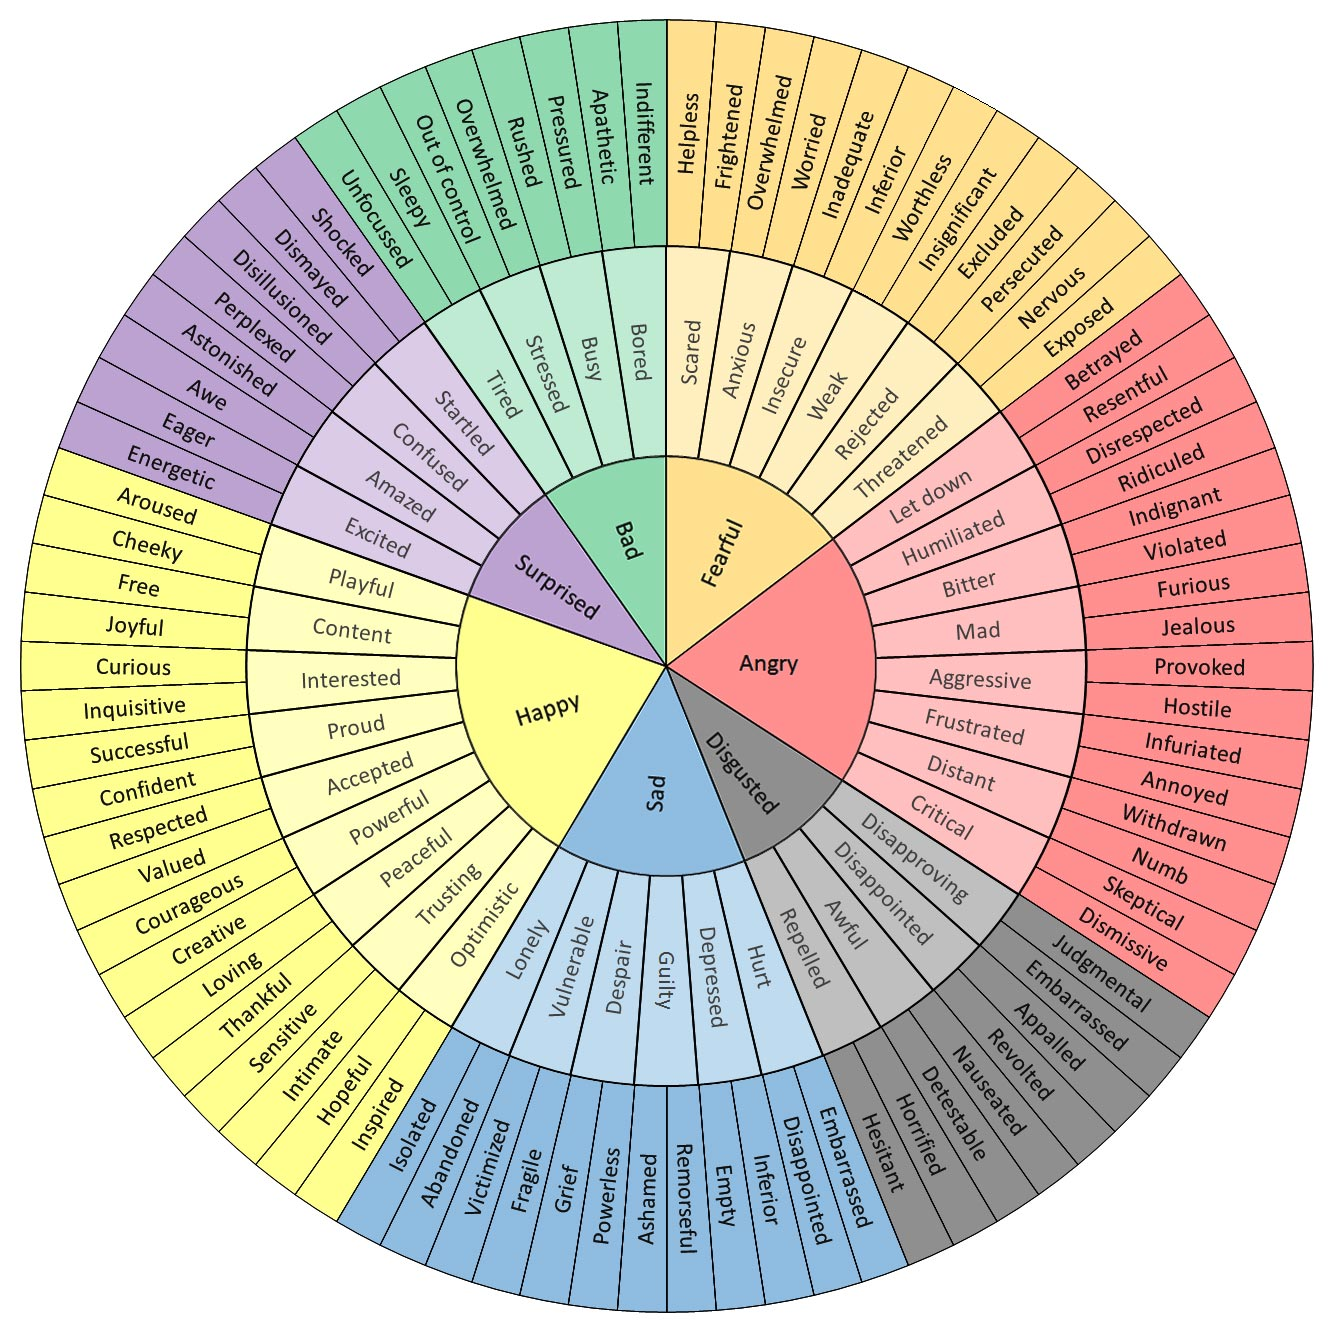
\includegraphics[width=0.95\textwidth]{WacuriFigures/EmotionWheel.jpg}
     \caption{Emotion Wheel (Copyright not yet obtained for this draft.)}
  \label{fig:emotionwheel}     
\end{figure}


As a convenience, we have provided one page of such a Journey Journal here.

\begin{tabular}{ |p{2cm}||p{2cm}|p{3cm}|p{1cm}|p{5cm}|  }
 \hline
 \multicolumn{5}{|c|}{Journey Journal} \\
 \hline
 Title& Date & Mood Words & Q (1-10) & Comments\\
  \hline
 \hline
 & & & & \\
 \hline 
 & & & & \\
 \hline 
 & & & & \\
 \hline 
 & & & & \\
 \hline 
 & & & & \\
 \hline 
 & & & & \\
 \hline 
 & & & & \\
 \hline 
  & & & & \\
 \hline
  \hline
\end{tabular}

\chapter{Applications}

The fundamental need to deepened human connections and wake people up
to curiosity is enough.

Nonetheless, we believe the Wacuri Method can help address a lot of
pressing problems, because connection and mindfulness are central to
wellness and health. Nobody who is lonely can really be happy. Nobody
who is cut off from others can be truly healthy.

Many of the problems we face, such as suicide, destructive behavior,
depression, addiction, and loneliness may be directly addressed by
creating friendships and shared human experience through
Journeys. Terminal illness, dementia, financial problems, and
frustrated ambition are indirectly aided by Journeys.

We believe from personal experience that the Wacuri Method may be
beneficial to those facing addiction, post-traumatic stress disorder,
loneliness and depression.  We seek to be able to fund research to
investigate this scientifically.

\section{Therapy}

We are both tantalized and highly motivated by the hints that the
Wacuri Method may be therapeutic for a number of troubles that plague
our modern society. Anything that might help depression, loneliness,
addiction, post-traumatic stress disorder, and the deep disconnection
people feel from each other and society is worth investigation.

Because the Wacuri Method always uses more than one person on Journey,
it is in a sense always deepening connection to others and to the
object of the Journey. We believe there is evidence that this
connection may be more important than any therapeutic effect that may
be achieved without a connection. It is possible that a machine or a
robot can massage our backs effectively; it is probably this will
never be as nice as a personal massage from a human hands.

Although in many cases the object of the Journey many not matter, it
seems possible that for therapeutic effect the object of the Journey
may be chosen to mean something particular to two people who may be
suffering in the same way. A Journey to the Transformation of Fear may
be especially therapeutic to two people suffering from anxiety. A
Journey to Brotherhood or Sisterhood may be especially meaningful to
soldiers suffering from PTSD.

Because Journey's can be emotionally powerful, we recommend in a
therapeutic setting that all participants agree on the object of the
Journey. It is possible that Jockey and the Journeyers may not feel
comfortable with a Journey today that they will be ready for
tomorrow. As always, a certain amount of trust must be constructed
between persons in a therapeutic setting.

\section{Productivity}

The Wacuri Method was specifically designed for the busy person who
can invest a limited amount of time in a mindfulness or meditation
practice. By using five-minute Journeys and short debriefs, the Wacuri
Method requires less time than other approaches. We have personally
found it to be equally effective to longer mindfulness training
exercises.

Our experience has been that a Journey refreshes the mind by
specifically and intensely, if briefly, transporting the mind from the
worries of the day and focusing it on a different object. As has been
often pointed out, the Journey matters more than the destination. The
act of participating in a Journey relieves the mind in several ways.

It is an act of listening, rather than speaking. The journeyer
fundamentally engages the imagination and the emotional capabilities,
without engaging the speaking capabilities. One experiences the
Journey, but does not have to instigate it.  Thus the leadership,
executive, scheduling, logical, and decisional processes get a respite
from a busy day. At the same time, the imagination (and perhaps
audiation), and emotional aspects of the mind are fully activated. A
Journey is thus an inversion of what most executives and managers do
during a busy day. The Journeyer is actively passive.

Many of us seek a running or weight-lifting partner not only to spot
us when we are benching or to keep us safe on the trail in the
predawn gloam.  Perhaps for the same reason we should have a
mindfulness partner.  At a more basic level, many of feel any
experience more intently if it is shared and witnessed by another
person. A Journey shared is not a Journey halved, but a Journey
doubled.  Social facilitation makes any simple task more efficient, and
nothing could be simpler than taking a Journey.

At a more practical level, most of us struggle to perform a
mindfulness practice on a daily basis in the presence of urgent and
unpredictable demands of a hectic day.  By committing to take a Journey
with another person, we motivate ourselves to keep our commitment. Most
of us do not want to let another person down if we can avoid it, and
feel badly when circumstances require us to do so.

\chapter{Related Scientific Research}

Siegel's book may be valuble \cite{siegel2007mindful}.


\chapter{Related Systems}

The Wacuri Method overlaps with mindfulness.  Mindfulness is focused
on taking things away. For example, it strives to rein in the
``monkey mind'' or the ``yapper'' that constantly intrudes with
verbal thoughts. The Wacuri Method, on the other hand, seeks
to awaken curiosity. Both systems strengthen the attentiveness
and powers of concentration, as represented in Figure \ref{fig:wacurivsmindfulness}. Mindfulness subtracts, Wacuri adds.

\begin{figure}
  \centering
     
\includegraphics[width=0.6\textwidth]{WacuriFigures/WacuriMindfulnessDiagram.png}
     \caption{Wacuri vs. Mindfulness}
  \label{fig:wacurivsmindfulness}     
\end{figure}

These are loose ideas and hypotheses that we have about metrics and connectedness:
\begin{itemize}
\item Five minutes more frequently is as valuable (or more) than longer meditations.
\item With practice, the time to get into a zone of beneficial mental state decreases.
\item Practice with the Wacuri Method increases curiosity, and, necessarily, presence.
  \item The impact of transmissions is scalar and may vary.
\end{itemize}



\appendix

\chapter{Some Journeys}
\label{sec:journeys}

Some of our best journeys
\begin{enumerate}
\item A Galaxy Cluster.mp3
\item Forgiveness (1).mp3
\item Journey to a Bumblebee (2).mp3
\item Journey to A Spiderweb+Music.mp3
\item Journey to Ancient Bacteria .mp3
\item Journey to Bioluminessence.mp3
\item Journey to Dark Matter and Dark Energy.mp3
\item Journey to Dark Matter and Dark Energy+Music.mp3
\item Journey to Forgiveness.mp3
\item Journey to The Birth of Stars+Music.mp3
\item Journey to the Birth of Stars.mp3
\item Journey to the Consciousness of Cells-MP3 File.mp3
\item Journey to The Elders+Music.mp3
\item Journey to the Illusion of Time .mp3
\item Journey to The Magnetic Field of the Earth+Music.mp3
\item Journey to The Magnetic Field of the Earth.mp3
\item Journey to The Song of Owls+Music.mp3
\item Journey to the Transformation of Fear.mp3
\item Journey-to-the-Elders.mp3
\end{enumerate}

\printbibliography

  \end{document}





TODO:  Get a quote fro here:

https://www.brainpickings.org/2017/04/05/erich-fromm-the-art-of-listening/
``How Language confers reality upon existence''

\url{http://marc.ucla.edu/workfiles/pdfs/MARC-mindfulness-research-summary.pdf}

\url{https://mail.google.com/mail/u/0/#search/dan+seigel/15cd0bac54934496?projector=1}
